% $Id: patches.tex 8166 2020-09-17 19:18:02Z mskala $

%
% MSK 013 patch ideas
% Copyright (C) 2020  Matthew Skala
%
% This program is free software: you can redistribute it and/or modify
% it under the terms of the GNU General Public License as published by
% the Free Software Foundation, version 3.
%
% This program is distributed in the hope that it will be useful,
% but WITHOUT ANY WARRANTY; without even the implied warranty of
% MERCHANTABILITY or FITNESS FOR A PARTICULAR PURPOSE.  See the
% GNU General Public License for more details.
%
% You should have received a copy of the GNU General Public License
% along with this program.  If not, see <http://www.gnu.org/licenses/>.
%
% Matthew Skala
% https://northcoastsynthesis.com/
% mskala@northcoastsynthesis.com
%

\chapter{Patch ideas}

The simplest way to patch the Middle Path is to not really patch it at
all.  Just running it by itself with no input except the front-panel
controls, it can produce a variety of different spectra for drones and
background pads.  Taking output from the ``sin'' and ``cos'' outputs of the
sine shaper gives a fake stereo effect.  Note that the V/octave inputs
normalize to the Eurorack CV bus when there are no cables plugged into the
front panel, so even without plugging in an input cable, the module can take
pitch control from somewhere else if used with modules like the Doepfer
A-185-1 that can send a control voltage to the bus.

\nopagebreak\noindent
{\hspace*{\fill}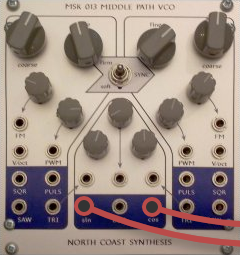
\includegraphics[scale=0.4]{mp-patch1.png}\hspace*{\fill}\par} 

Here are two independent subtractive East Coast-style voices in an 84HP
Eurorack row, using the Middle Path as a dual general-purpose VCO.  Pitch CV
from the MIDI interface drives the two V/oct inputs of the Middle Path, as
well as the pitch CV inputs of the filters, which in this case are Coiler
VCFs.  Gate CV drives two ADSR envelope generators for each voice, which
control the filters and VCAs.

\nopagebreak\noindent
{\hspace*{\fill}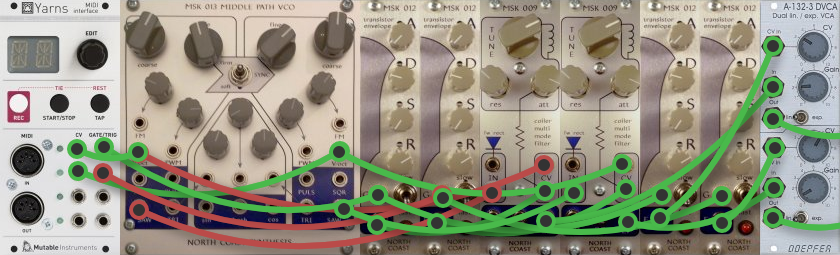
\includegraphics[width=\linewidth]{mp-patch2.png}\hspace*{\fill}\par} 

A more full-featured subtractive patch can use both oscillators of the Middle
Path in a single voice, as well as showcasing a couple of other North Coast
modules.  Pitch CV goes through a Dual Octave Switch, which allows for
easily shifting either oscillator up or down during performance.  The Fixed
Sine Bank provides PWM to one oscillator and FM to the other.  The PWM on
the first oscillator won't be audible in its triangle output, which is the
default normalized to the sine shaper, but using firm sync mode would allow
the PWM to have an effect, or we can patch the PULS output into one of the
sine shaper's inputs as shown.  The MIDI gate drives two ADSR envelopes, one
for the filter and one for the VCA.  The Doepfer VCA used here has two audio
inputs so we patch in the low-pass and band-pass outputs of the filter to
provide some mixing options.

\nopagebreak\noindent
{\hspace*{\fill}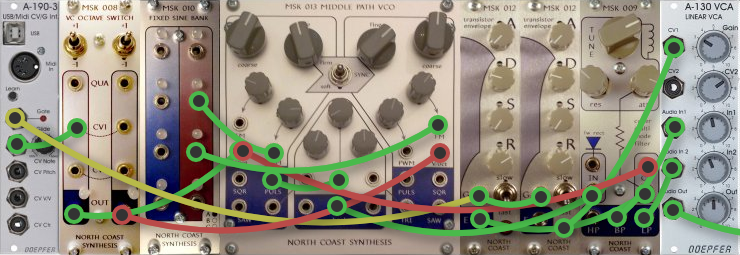
\includegraphics[width=\linewidth]{mp-patch3.png}\hspace*{\fill}\par} 

The sine shaper can process an external input if it's raised to an
appropriate level.  Depending on how hard it's driven, it can range from
just a mild enhancement of odd harmonics, through tube-like foldback, into
complete wavefolding.  In this example, the three outputs from the shaper go
through a Transistor Mixer to mix them down and provide some additional
distortion options of its own.  Turning down the levels on the Transistor
Mixer allows it to knock the level back down to a typical audio ``line
level'' for further connection to non-Eurorack equipment.

\nopagebreak\noindent
{\hspace*{\fill}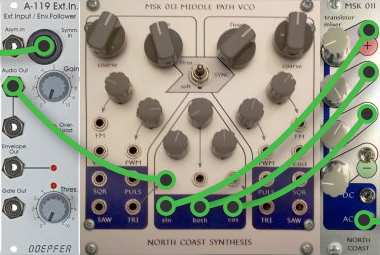
\includegraphics[scale=0.4]{mp-patch5.png}\hspace*{\fill}\par} 

Here's a West Coast-style voice emphasizing the modulation effect of
the Middle Path sine shaper, with a Leapfrog VCF serving as a low-pass
gate.  With the pitch CV patched into the left oscillator as shown, it will
affect both, so the carrier and modulator will track each other.  Another
possibility would be to patch it in on the right instead; then it will only
affect that oscillator while the other one remains at an unchanging
frequency set by the front-panel controls or the Eurorack bus CV.

Through-zero phase modulation is achieved when the slope of the
modulator waveform exceeds that of the carrier, so that the phase input to
the sine shaper runs backwards.  Tune one oscillator to a higher frequency
than the other, and adjust the lower-frequency oscillator to a higher input
level on the sine shaper, to get through-zero with this patch.  The envelope can
drive just the filter cutoff for a pure low-pass gate effect, or patch it into
the Leapfrog's built-in VCA also for a more extreme cutoff of amplitude as
well as frequency (which allows
tuning the filter higher).

\nopagebreak\noindent
{\hspace*{\fill}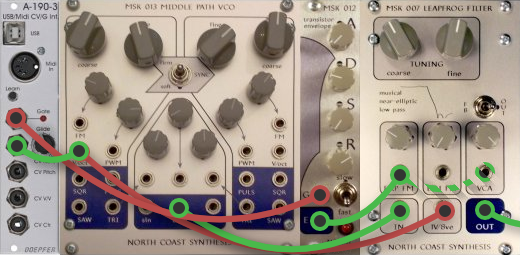
\includegraphics[scale=0.4]{mp-patch4.png}\hspace*{\fill}\par} 

Quadrature outputs on the Middle Path make it a building block for
Bode-type frequency shifter patches.  In this example, the master (left)
oscillator with its PWM knob turned all the way counterclockwise gives two
square waves 90$^\circ$ apart in phase on its SQR and PULS outputs.  Those drive
two of the inputs on the Doepfer dual ring modulator.  The master
oscillator's contribution to the sine shaper input is turned off.  Meanwhile
the slave (right) oscillator drives the sine shaper, whose ``sin'' and
``cos'' outputs also go into the dual ring modulator.  A Dual Octave Switch
functioning as adder/subtractor gives two different mixes of the ring
modulator outputs corresponding to frequency shift up and down.  If only one
of those were desired, a plain unity mixer would suffice.

Because of the approximations involved in this frequency-shift patch, such
as using square waves instead of sines for one of the analytic signals, the
result will not be a pure frequency shifted spectrum; some components will
shift in the ``wrong'' direction, or not be filtered out.  It'll still sound
interesting, though.  To get a purer result, patch the sawtooth output of
the slave oscillator into the corresponding shaper input, overriding the
normalization to the triangle output.  Then with the level adjusted to make
them as close to pure sine waves as possible, the ``sin'' and ``cos''
outputs will be just quadrature sine waves suitable for a pure frequency
shift.  That same technique can also be used for making the Middle Path a
quadrature sine oscillator in a more complicated frequency shifter
with external input, a Hilbert transformer, and so on.

\nopagebreak\noindent
{\hspace*{\fill}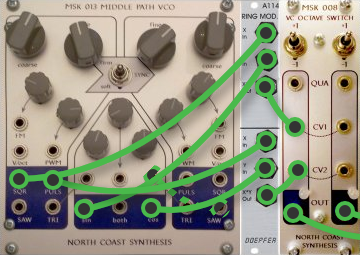
\includegraphics[scale=0.4]{mp-patch6.png}\hspace*{\fill}\par} 

When tuning the Middle Path to match its V/octave reference point to some
known value, for instance to match MIDI notes, it's convenient to listen to
the beat frequencies in the sine shaper.  Here, the Mutable CVpal in
``turbocharged monophonic mode'' (MIDI channel 2) produces a pitch CV and
also a square wave at the corresponding frequency.  We patch the pitch CV to
the Middle Path V/octave input (affecting both oscillators), the square wave
to one of the sine shaper inputs, and then listen to the sine shaper output
and play with the shaper levels and oscillator tuning.  Bringing up one
oscillator at a time against the square wave makes the beat frequency
between them strongly audible, at which point it's easy to tune the
oscillator to match the MIDI interface within a fraction of a Hz.  Other
things instead of a CVpal could easily be used as the reference here -- such
as other oscillators in a multi-oscillator system.

\nopagebreak\noindent
{\hspace*{\fill}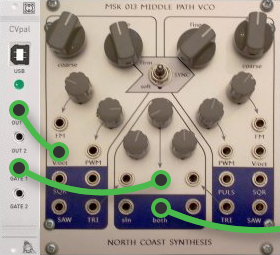
\includegraphics[scale=0.4]{mp-patch7.png}\hspace*{\fill}\par} 
